% Drawing 147/08-2 -- folder 147, batch 08, archive page 142 (PDF page 143).
% Transcription: Une bande courbe (le voisinage tubulaire), traversée par une courbe centrale ; en deux points, une branche transverse coupe la courbe, et autour de chaque point quatre quadrants hachurés ; une flèche désigne les branches comme $\Theta_{D',Y}$.
% Kind: tubular neighbourhood with transverse branches and hatched quadrants. Method 2 (schematic redraw from the facsimile). Status: ok.
% Notes: A curved band (the tubular neighbourhood) crossed by a central curve; at two points a transverse branch cuts the curve, with four hatched quadrants round each point (drawn as alternate hatched sectors); an arrow points to the branches as Theta_{D',Y}. The band is cut by the right edge of the drawing on the page; the transverse lines of the band are drawn at regular steps.
% Coordinates: 1 unit = 1 mm = 1/100 of the crop width (bbox in page fractions: [0.188, 0.311, 0.68, 0.459]).
% Redrawn by Claude (claude-opus-5-5), issue #73, 2026-11-07; not checked by a human; not compiled (no TeX in the session).
% Rights: reproduces part of the work -- behind RENDER_TRANSCRIPTS, never published by itself.
\documentclass[tikz,border=3pt]{standalone}
\usepackage{amsmath,amssymb}
\usetikzlibrary{patterns,arrows.meta}
\tikzset{pencil/.style={black!45}, struck/.style={black!35}, mark/.style={circle,draw,inner sep=1.3pt}, pt/.style={circle,fill,inner sep=0.9pt}, opt/.style={circle,draw,fill=white,inner sep=1.1pt}}
\begin{document}
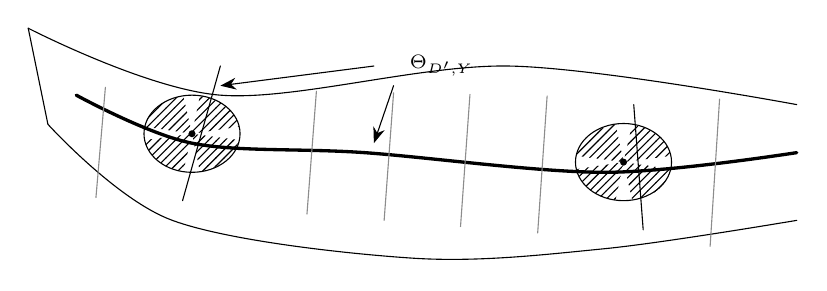
\begin{tikzpicture}[x=1mm,y=1mm,line cap=round,line join=round,font=\scriptsize]
\draw plot[smooth, tension=0.55] coordinates {(2.4,-9.8) (26.8,-18.3) (63.4,-14.6) (100,-19.5)};
\draw plot[smooth, tension=0.55] coordinates {(4.9,-22) (20.7,-34.2) (51.2,-39) (75.6,-37.8) (100,-34.2)};
\draw (2.4,-9.8) -- (4.9,-22);
\draw[very thick] plot[smooth, tension=0.55] coordinates {(8.5,-18.3) (23.2,-24.4) (45.1,-25.6) (75.6,-28.1) (100,-25.6)};
\draw[pencil] (12.2,-17.3) -- (11,-31.3);
\draw[pencil] (39,-17.8) -- (37.8,-33.4);
\draw[pencil] (48.8,-18) -- (47.6,-34.2);
\draw[pencil] (58.5,-18.2) -- (57.3,-35);
\draw[pencil] (68.3,-18.4) -- (67.1,-35.8);
\draw[pencil] (90.2,-18.8) -- (89,-37.5);
\draw (23.2,-23.2) ellipse[x radius=6.1, y radius=4.9];
\fill[pattern=north east lines] (23.2,-23.2) -- (29.2,-22.3) -- (28.9,-21.5) -- (28.5,-20.7) -- (27.8,-20) -- (27.1,-19.4) -- (26.2,-19) -- (25.3,-18.6) -- (24.2,-18.4) -- cycle;
\fill[pattern=north east lines] (23.2,-23.2) -- (22.1,-18.4) -- (21.1,-18.6) -- (20.1,-19) -- (19.3,-19.4) -- (18.5,-20) -- (17.9,-20.7) -- (17.4,-21.5) -- (17.2,-22.3) -- cycle;
\fill[pattern=north east lines] (23.2,-23.2) -- (17.2,-24) -- (17.4,-24.8) -- (17.9,-25.6) -- (18.5,-26.3) -- (19.3,-26.9) -- (20.1,-27.4) -- (21.1,-27.8) -- (22.1,-28) -- cycle;
\fill[pattern=north east lines] (23.2,-23.2) -- (24.2,-28) -- (25.3,-27.8) -- (26.2,-27.4) -- (27.1,-26.9) -- (27.8,-26.3) -- (28.5,-25.6) -- (28.9,-24.8) -- (29.2,-24) -- cycle;
\draw (26.8,-14.6) -- (22,-31.7);
\node[pt] at (23.2,-23.2) {};
\draw (78,-26.8) ellipse[x radius=6.1, y radius=4.9];
\fill[pattern=north east lines] (78,-26.8) -- (84.1,-26) -- (83.8,-25.2) -- (83.3,-24.4) -- (82.7,-23.7) -- (82,-23.1) -- (81.1,-22.6) -- (80.1,-22.3) -- (79.1,-22) -- cycle;
\fill[pattern=north east lines] (78,-26.8) -- (77,-22) -- (76,-22.3) -- (75,-22.6) -- (74.1,-23.1) -- (73.4,-23.7) -- (72.8,-24.4) -- (72.3,-25.2) -- (72,-26) -- cycle;
\fill[pattern=north east lines] (78,-26.8) -- (72,-27.7) -- (72.3,-28.5) -- (72.8,-29.3) -- (73.4,-30) -- (74.1,-30.6) -- (75,-31.1) -- (76,-31.4) -- (77,-31.6) -- cycle;
\fill[pattern=north east lines] (78,-26.8) -- (79.1,-31.6) -- (80.1,-31.4) -- (81.1,-31.1) -- (82,-30.6) -- (82.7,-30) -- (83.3,-29.3) -- (83.8,-28.5) -- (84.1,-27.7) -- cycle;
\draw (79.3,-19.5) -- (80.5,-35.4);
\node[pt] at (78,-26.8) {};
\node[inner sep=1pt] at (54.9,-14.6) {\scriptsize $\Theta_{D',Y}$};
\draw[-{Stealth[length=2mm]}] (46.3,-14.6) -- (26.8,-17.1);
\draw[-{Stealth[length=2mm]}] (48.8,-17.1) -- (46.3,-24.4);
\end{tikzpicture}
\end{document}
